
\chapter{Desenvolvimento}\label{cap:desenvolvimento}

Como referenciado, a correspondência entre SSA e programação funcional já foi explorada por vários trabalhos que buscaram entender como extrair valor deste fato. Notoriamente, \citeonline{rigon2020inferring} exploram esta correspondência ao propor o núcleo de uma linguagem pseudo-imperativa com sistema de tipo e efeitos baseados no trabalho de \citeonline{leijen2014koka} usando a forma SSA traduzida do código em Koka.

O presente trabalho implementa uma proposta de extensão do trabalho de \citeonline{rigon2020inferring}, agora traduzindo código genérico para programação funcional (em ANF), a partir da representação intermediária da LLVM. Levando a possibilidade de, no futuro, ser pesquisada a inferência de efeitos em código em LLVM-IR, consequentemente código gerado a partir de linguagens imperativas.

Uma das propostas de valor deste trabalho é apresentada na Figura \ref{fig:proposta}, demonstrando a possibilidade de tradução de código arbitrário para código funcional. A partir de código em alguma linguagem fonte como C, C++ ou Rust, a LLVM é utilizada para gerar a LLVM-IR em forma SSA. A representação intermediária gerada é então usada como entrada para o método proposto nesse trabalho, que faz a tradução da representação intermediária da LLVM para código funcional em forma ANF na linguagem Haskell. Porém, essa é ainda uma exploração inicial dessa tradução, já que nesse trabalho é interpretado somente um subconjunto da representação intermediária da LLVM.

\begin{figure}[h]
    \centering
    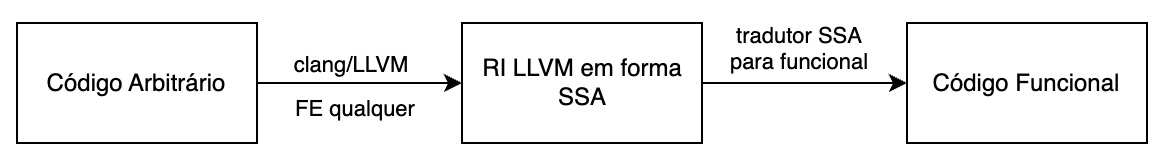
\includegraphics[width=\textwidth]{Imagens/proposta2.jpg}
    \caption{Diagrama da Proposta do Sistema de Tradução}\
    \label{fig:proposta}
    \small{Fonte: O autor}
\end{figure}

O método de tradução proposto neste trabalho foi implementado em duas fases: inicialmente criando um \emph{parser} (analisador sintático) para um subconjunto da representação intermediária da LLVM, e então desenvolvendo uma adaptação do método descrito por \citeonline{ssaToAnf} para traduzir a LLVM-IR em forma SSA para uma representação intermediária similar à ANF que é apresentada como código em linguagem Haskell. O objetivo da geração do código na sintaxe de Haskell é facilitar a validação do trabalho, uma vez que dessa forma programas que não apresentam efeitos colaterais poderão ser executados.

\section{\emph{Parser} da LLVM-IR}

A primeira etapa para a tradução é a implementação de um \emph{parser} da LLVM-IR para que, com base no código interpretado, a tradução seja aplicada. Deste modo, a gramática usada para a interpretação foi desenvolvida com base em exemplos gerados usando o \emph{clang} em código C++, e com base na documentação de referência da linguagem que é fornecida pela LLVM\footnote{https://llvm.org/docs/LangRef.html}.

Visto que a LLVM-IR conta com diversas funcionalidades de alto e baixo nível, no código podem ser geradas diversas informações como: metadados, informação para depuração, \emph{flags} de otimização, etc \cite{llvmLangRef}. Entre estas, há muitas operações, palavras reservadas e funções nativas que não são úteis ou fogem do escopo deste trabalho. Devido a isso e ao tempo disponível para desenvolvimento, um subconjunto da linguagem intermediária foi selecionado. Nesse subconjunto o escopo global só permite definição de funções, sem variáveis ou demais dados globais. Ademais, para simplificar o escopo deste trabalho, constantes foram limitadas somente a numerais de tipos inteiros de qualquer tamanho.

\begin{figure}[h]
\begin{center}
\large
\begin{tabular}{r@{\ \ }c@{\ \ }l}
    $p$ & ::= & $\textbf{define} \ t \ x \ \textbf{(} \ \overline{t \ \ x} \ \textbf{)}\ \textbf{\{}\ \overline{b}\ \textbf{\}}$ \\
    $b$ & ::= & $x$ \ \textbf{:} \ $\overline{\phi}$ \ $\overline{s}$ \ $f$ \\
    $\phi$ & ::= & $x$ \ \textbf{=} \ $\textbf{phi}$ \ $t$ \ $\overline{a}$ \\
    $s$ & ::= & $x$ \ $\boldsymbol{=}$ \ $o$ \ $|$ \ $x$ \ $\boldsymbol{=}$ \ $q$ \\
    $q$ & ::= & \textbf{call} \ $t$ \ $x$ \ $\textbf{(} \ \overline{t \ v} \ \textbf{)}$ \\
    $f$ & ::= & \textbf{br} \ $t$ \ $x$ \ $|$ \ \textbf{br} \ $t$ \ $v$ \ \textbf{,} \ $t$ \ $x$ \ \textbf{,} \ $t$ \ $x$ $|$ \ \textbf{ret} \ $t$ \ $v$ \\
    % $\overline{a}$ & ::= & $a$ \ \textbf{,} \ $\overline{a}$ \\
    % $\overline{x}$ & ::= & $t$ \ $x$ \ \textbf{,} \ $\overline{x}$ \ $|$ \ $t$ \ $x$ $|$ \ $\epsilon$\\
    $a$ & ::= & $\textbf{[}$ \ $v$ \ \textbf{,} \ $x$ \ \textbf{]} \\
    $o$ & ::= & $\beta$ \ $t$ \ $v$ \ \textbf{,} \ $v$ \ $|$ \\ 
    & & $\mathbf{icmp}$ \ $\tau$ \ $t$ \ $v$ \ \textbf{,} \ $v$ \ $|$ \\
    & & \textbf{select} \ $t$ \ $v$ \ \textbf{,} \ $t$ \ $v$ \ \textbf{,} \ $t$ \ $v$ \ $|$  \\ 
    & & $\mu$ \ $t$ \ $v$ \ \textbf{to} \ $t$ \\
    $v$ & ::= & $x$ $|$ $c$ \\
    $t$ & $\in$ & \emph{tipos nativos da LLVM}  \\
    $x$ & $\in$ & \emph{variáveis locais ou globais} \\
    $c$ & $\in$ & \emph{constantes} \\
    $\beta$ & $\in$ & \emph{operações binárias da LLVM} \\
    $\tau$ & $\in$ & \emph{opções de comparação da LLVM} \\
    $\mu$ & $\in$ & \emph{operações de conversão da LLVM} \\
\end{tabular}
\caption{Gramática de interpretação da LLVM-IR}
\label{fig:llvm-ir-gramatica}
\small{Fonte: O autor}
\end{center}
\end{figure}

Conforme a gramática presente na Figura \ref{fig:llvm-ir-gramatica}, os procedimentos em LLVM-IR tratados nesse trabalho são na seguinte forma: a definição de uma função se dá pelo seu tipo, nome, os seus parâmetros, e os blocos da forma SSA. Os blocos são definidos por seu \emph{label} e devem conter, nessa ordem, uma sequência de $\phi$s, em seguida as declarações de variáveis, e por último um \emph{jump} no fluxo de controle (por exemplo, retorno ou \emph{branch}). É determinado que todos os blocos e argumentos precisam ter um \emph{label}, ou seja, precisam ser nomeados. Nesta gramática o não terminal $o$ representa as operações nativas da LLVM, nas quais estão compreendidas operações matemáticas, de comparação, conversão, entre outras. Essas operações nativas foram mapeadas e traduzidas para operações correspondentes em linguagem Haskell, para que o código gerado possa ser executado. Na Seção \ref{cap:desenvolvimento-traducao} há mais detalhes sobre como essas operações foram traduzidas. Observa-se também que na LLVM-IR não há necessidade de um terminador de linha como ";" \ ou até mesmo uma nova linha para a próxima instrução. Devido a isso, a gramática não contém nenhum terminal pontuando o fim de uma linha.

A Figura \ref{fig:exemplo-entrada} apresenta um exemplo de código bem formatado que é gerado pela gramática definida. Neste exemplo foram removidas \emph{flags} de otimização, informação para depuração e outras informações que são ignoradas durante a análise léxica. Nota-se que os tipos fazem parte da estrutura do código na linguagem de entrada. Posteriormente esses tipos são desconsiderados ao gerar a representação ANF em código. Ao final desta etapa obtêm-se uma representação em memória do SSA interpretado, com toda a informação necessária para fazer a tradução descrita na Seção \ref{cap:desenvolvimento-traducao}.

\begin{figure}
\centering
\lstset{xleftmargin=.25\textwidth}
\begin{lstlisting}[language=llvm,style=nasm]
define i32 @factorial(i32 %0) {
1:
  br label %2

2:
  %3 = phi i32 [ 1, %1 ], [ %8, %6 ]
  %4 = phi i32 [ %0, %1 ], [ %7, %6 ]
  %5 = icmp slt i32 %4, 2
  br i1 %5, label %9, label %6

6:
  %7 = add nsw i32 %4, -1
  %8 = mul nsw i32 %3, %4
  br label %2

9:
  %10 = mul nsw i32 %3, 1
  ret i32 %10
}
\end{lstlisting}
\caption{Exemplo de Código de Entrada Válido}
\label{fig:exemplo-entrada}
\small{Fonte: O autor}
\end{figure}

\section{ANF Gerado}\label{sec:desenvolvimento-anf}

A gramática ANF descrita nesta seção busca esclarecer e facilitar as notações e entendimento do leitor. Todavia, é necessário destacar que o código de saída do método desenvolvido é em Haskell e será melhor abordado no final da Seção \ref{cap:desenvolvimento-traducao}.

Recapitulando sobre ANF, pode-se frasear as suas restrições em: argumentos de funções devem ser valores atômicos (constantes ou variáveis), e resultados de aplicações devem ser imediatamente capturados por uma variável dentro de um \emph{let}. A gramática definida como saída visa garantir que estas restrições sejam diretamente atingidas somente pelo fato do programa pertencer às produções da gramática livre de contexto.

A forma ANF definida na gramática da Figura \ref{fig:gramatica-saida} é uma variante da ANF original, na qual foram adicionadas algumas funcionalidades, por exemplo: as funções podem ter mais de um argumento, há operações primitivas (operações matemáticas e bit a bit) e condicionais. As produções sobre o não terminal $o$ são as traduções das operações nativas da LLVM para sintaxe do Haskell que, para efeitos desse trabalho, puramente retornam o valor resultante da operação. A tradução dessas operações é melhor descrita na seção seguinte, e suas produções podem ser vistas na coluna da direita da Tabela \ref{tab:traducao-operacoes}.

\begin{figure}[h]
\begin{center}
\large
\begin{tabular}{r@{\ \ }c@{\ \ }l}
    $f$ & ::= & $\textbf{def} \ \ x \ \ \boldsymbol{=} \ \ \boldsymbol{\lambda} \ \overline{x} \ . \ \textbf{let} \ \ l \ \ \textbf{in} \ \ 
    x \ \ \overline{v}$ \\
    $l$ & ::= & $x \ \ \boldsymbol{=} \ \ \boldsymbol{\lambda} \ \overline{x} \ . \ \textbf{let} \ \ \overline{d} \ \ \overline{l} \ \ \textbf{in} \ \ j$ \\
    $d$ & ::= & $x \ \ \boldsymbol{=} \ \ e$ \\
    $e$ & ::= & $v \ \ | \ \ x \ \ \overline{v} \ \ | \ \ o \ \ \overline{v}$ \\
    $j$ & ::= & $v \ \ \overline{v} \ \ | \ \ \textbf{if} \ \ v \ \boldsymbol{\neq} \ \mathbf{0 \ \ then} \ \ v \ \ \overline{v} \ \ \textbf{else} \ \ v \ \ \overline{v}$ \\
    $v$ & ::= & $x$ $|$ $c$ \\
    $o$ & $\in$ & \emph{operações nativas da LLVM traduzidas} \\
    $x$ & $\in$ & \emph{variáveis} \\
    $c$ & $\in$ & \emph{constantes} \\
\end{tabular}
\caption{Gramática do ANF Gerado como Saída}
\label{fig:gramatica-saida}
\small{Fonte: O autor}
\end{center}
\end{figure}

Sobre $f$, está a produção da função em ANF que irá corresponder a função a ser traduzida da forma SSA, que fundamentalmente contém a definição da função traduzida do bloco inicial e a chamada para esse bloco inicial. As produções sobre o não terminal $j$ são as chamadas de cauda das funções em ANF, chamadas podem ser para um valor (retorna o valor), outra função, ou uma condicional. A condicional é traduzida diretamente para $v \ \ \mathbf{\neq 
\ 0}$ para ser uma tradução mais direta da instrução de \verb|br| da LLVM-IR.

\section{Processo de tradução}\label{cap:desenvolvimento-traducao}

O procedimento de tradução desenvolvido foi uma adaptação da tradução descrita por \citeonline{ssaToAnf}. O código em LLVM-IR na forma SSA é interpretado e utilizado como entrada para $\mathcal{F}$ (Figura \ref{fig:traducao}), dando como saída o código em ANF seguindo a gramática livre de contexto da Tabela \ref{tab:traducao-operacoes}.

Ao fazer a tradução de SSA para ANF, inicialmente há de ser tratada de uma diferença fundamental entre SSA e ANF quanto à explicitude do escopo das variáveis no código. Em ANF o escopo é explícito na estrutura do código, ou seja, se uma variável existe em uma função, ela existe em todas as funções que são aninhadas nessa função, e não existe antes ou depois da definição da função. Em SSA, blocos que vêm antes no código, podem usar variáveis que ainda não foram definidas, contanto que em tempo de execução aquela variável exista e a definição da variável domine seus usos. Em outras palavras, em SSA o escopo é determinado pelo grafo de fluxo de controle, que não é explícito na estrutura do código e sim implícito nos seus \emph{jumps}. Por isso, para que a tradução entre ambos seja feita, é utilizado o conceito de árvores de dominância (Definição \ref{def:dom-tree}), que é calculada sobre o grafo de fluxo de controle da forma SSA. A Figura \ref{fig:graph-vs-dom-factorial} contém um exemplo do CFG e da árvore de dominância do código da Figura \ref{fig:exemplo-entrada}.

\begin{figure}[H]
\centering
\begin{subfigure}{.5\textwidth}
  \centering
  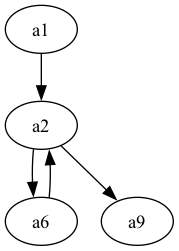
\includegraphics[width=.4\linewidth]{Imagens/fact-desenv-graph.png}
  \caption{Grafo de fluxo de controle}
  \label{fig:sub1}
\end{subfigure}%
\begin{subfigure}{.5\textwidth}
  \centering
  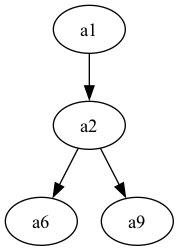
\includegraphics[width=.4\linewidth]{Imagens/fact-desenv-dominance.png}
  \caption{Árvore de dominância}
  \label{fig:sub2}
\end{subfigure}
\caption{CFG e Árvore de Dominância do Código da Figura \ref{fig:exemplo-entrada}}
\label{fig:graph-vs-dom-factorial}
\small{Fonte: O autor}
\end{figure}

A Figura \ref{fig:traducao} apresenta o método de tradução desenvolvido. Sobre a notação utilizada, de mesma forma que as produções gramaticais anotadas com \emph{overline}, funções anotadas com \emph{overline} querem dizer que aquela função é aplicada ponto a ponto. 

A tradução começa por $\mathcal{F}$, que recebe toda a função em SSA e irá retornar a função em ANF, os argumentos são os mesmos da função em SSA. Em termos, a função traduzida contém a tradução do primeiro bloco e a chamada para a função traduzida desse primeiro bloco. Por isso, após em $\mathcal{F}$, $\mathcal{F}_b$ é chamada e faz a tradução do bloco inicial, a qual estarão aninhadas, direta ou indiretamente, todas as demais funções, uma vez que o bloco inicial domina todos os demais. A chamada de cauda da função inicial é a chamada de cauda para função correspondente ao bloco inicial e é o ponto inicial da execução.

A tradução dos blocos em $\mathcal{F}_b$, de mesma forma, é feita retornando uma função em ANF. Os argumentos são determinados pelos $\phi$s do bloco em SSA ($\mathcal{F}_\phi$). Um argumento é gerado para cada $\phi$, e o nome deste argumento é o nome da variável ao qual o resultado da instrução \verb|phi| é atribuído. Após os $\phi$s, o bloco em SSA contém uma lista de definições de variáveis, as quais são traduzidas em $\mathcal{F}_s$. No escopo do bloco sendo traduzido são aninhadas as funções referentes aos blocos dominados imediatamente por este, por isto chama-se recursivamente $\mathcal{F}_b$ para os blocos filhos do bloco sendo traduzido. Toda função em ANF terá uma chamada de cauda, e as chamadas em ANF são traduzidas a partir do \emph{jump} da forma SSA. Se o \emph{jump} da LLVM-IR é o retorno de um valor, esse valor é retornado na função; se esse \emph{jump} é um \emph{branch} sem condicional para outro bloco, a função traduzida referente a este outro bloco é chamada; se há um \emph{branch} condicional na forma SSA, esse \emph{branch} é traduzido para uma condicional na forma ANF.

\begin{figure}[H]
    \begin{tabular}{ l }
    \textbf{Função de Tradução} \\
    $\mathcal{F}(\textbf{define}$ \ $t$ \ $x$ \ $\boldsymbol{(}$ \ $\overline{t \ x}$ \ $\boldsymbol{)}$ \ \textbf{\{} $\overline{b}$ $\textbf{\}})$ \ = \\
    \qquad \textbf{def} \ $x$ \ $\boldsymbol{=}$ \ $\boldsymbol{\lambda}$ $\overline{x}$ \textbf{.let} \ $\overline{\mathcal{F}_b(b)}$ \ \textbf{in} \ $\mathcal{F}_i(b)$ \\
    \qquad onde $b$ = nó inicial de $\overline{b}$ \\ \\
    \textbf{Tradução de um Bloco Básico} \\
    $\mathcal{F}_b(x$ \ \textbf{:} \ $\overline{\phi}$ \ $\overline{s}$ \ $f)$ \ = \\
    \qquad $x$ \ $\boldsymbol{=}$ \ $\boldsymbol{\lambda}$ $\overline{\mathcal{F}_\phi(\phi)}$ \textbf{.let} \ $\overline{\mathcal{F}_s(s)}$ \ $\overline{\mathcal{F}_b(b^\prime)}$ \ \textbf{in} \ $\mathcal{F}_f(x, f)$ \\
    \qquad onde $\overline{b'}$ = nós filhos de $x$ na árvore de dominância \\ \\
    \textbf{Tradução das Declarações} \\
    $\mathcal{F}_s(x \ \boldsymbol{=} \ \beta$ \ $t$ \ $v_1$ \ \textbf{,} \ $v_2)$ \ = \ $x$ \ $\boldsymbol{=}$ \ $v_1$ \ \`{}$\beta$\`{} \  $v_2$ \\
    $\mathcal{F}_s(x \ \boldsymbol{=} \ \mathbf{icmp}$ \ $\tau$ \ $t$ \ $v_1$ \ \textbf{,} \ $v_2)$ \ = \ $x$ \ $\boldsymbol{=}$ \ \textbf{if} \ $v_1$ \ $\tau$ \ $v_2$ \ \textbf{then \ 1 \ else \ 0} \\
    $\mathcal{F}_s(x \ \boldsymbol{=} \ \textbf{select}$ \ $t_c$ \ $v_c$ \ \textbf{,} \ $t_1$ \ $v_1$ \ \textbf{,} \ $t_2$ \ $v_2)$ \ = \ $x$ \ $\boldsymbol{=}$ \ \textbf{if} \ $v_c$ \textbf{/= \ 0 \ then} \ $v_1$ \ \textbf{else} \ $v_2$ \\
    $\mathcal{F}_s(x$ \ $\boldsymbol{=}$ \ $\mu$ \ $t_1$ \ $v$ \ \textbf{to} \ $t_2)$ \ = \ $x$ \ \textbf{=} \ $v$ \\
    $\mathcal{F}_s(x_1$ \ $\boldsymbol{=}$ \ \textbf{call} \ $t$ \ $x_2$ \ $\textbf{(} \ \overline{t \ v} \ \textbf{)})$ \ = \ $x_1$ \ $\boldsymbol{=}$ \ $x_2$ \ $\overline{v}$ \\
    onde $\beta$ e $\tau$ são traduzidos segundo a Tabela \ref{tab:traducao-operacoes} \\ \\
    \textbf{Tradução de um Jump} \\
    $\mathcal{F}_f(x_1$, $\textbf{br}$ \ $t$ \ $x_2)$ \ = \\
    \qquad $x_2$ \ $\overline{\mathcal{F}_p(x_1, \phi)}$ \\
    \qquad onde $x_2$ \ \textbf{:} \ $\overline{\phi}$ \ $\overline{s}$ \ $f$ = bloco com label $x_2$ \\ \\
    $\mathcal{F}_f(x_1$, \textbf{br} \ $t$ \ $v$ \ \textbf{,} \ $t$ \ $x_2$ \ \textbf{,} \ $t$ \ $x_3)$ \ = \\
    \qquad \textbf{if} \ $v$ \ \textbf{$\boldsymbol{\neq}$ \ 0 \ then} \ $x_2$ \ $\overline{\mathcal{F}_p(x_1, \phi_2)}$ \ \textbf{else} \ $x_3$ \ $\overline{\mathcal{F}_p(x_1, \phi_3)}$ \\
    \qquad onde $x_2$ \ \textbf{:} \ $\overline{\phi_2}$ \ $\overline{s_2}$ \ $f_2$ = bloco com label $x_2$ \\
    \enspace \quad \qquad e $x_3$ \ \textbf{:} \ $\overline{\phi_3}$ \ $\overline{s_3}$ \ $f_3$ = bloco com label $x_3$ \\ \\
    $\mathcal{F}_f(x_1$, \textbf{ret} \ $t$ \ $v)$ \ = \ $v$ \\ \\
    \textbf{Encontra os Argumentos de uma Chamada no $\phi$ do Bloco Alvo} \\
    $\mathcal{F}_p(x_1$, $x_2$ \ $\boldsymbol{=}$ \ $\textbf{phi}$ \ $t$ \ $\overline{a})$ \ = \\
    \qquad $v$ \\
    \qquad onde $\textbf{[}$ \ $v$ \ \textbf{,} \ $x_1$ \ \textbf{]} é um elemento de $\overline{a}$ \\ \\
    \textbf{Retorna a Variável Correspondente ao $\phi$} \\
    $\mathcal{F}_\phi(x$ \ $\boldsymbol{=}$ \ $\textbf{phi}$ \ $t$ \ $\overline{a})$ \ = \ $x$ \\ \\
    \textbf{Retorna o \emph{Label} do Bloco} \\
    $\mathcal{F}_i(x$ \ \textbf{:} \ $\overline{\phi}$ \ $\overline{s}$ \ $f)$ \ = \ $x$ \\
    \end{tabular}
    \begin{center}
    \caption{Procedimento de Tradução}
    \label{fig:traducao}
    \small{Fonte: O autor}
    \end{center}
\end{figure}

Em $\mathcal{F}_j$, os argumentos para as chamadas de cauda das funções traduzidas são buscados nos $\phi$s do bloco destino com base no \emph{label} do bloco origem. Por exemplo, se o bloco de \emph{label} $a$ tem um \emph{jump} para o bloco de \emph{label} $b$, e $\overline{\phi}_b$ é o conjunto de $\phi$s de $b$. Então, para cada $\phi_b$ é buscado o argumento $\textbf{[} \ v \ \textbf{,} \ \ l \ \textbf{]}$ onde $l = b$, retornando que o valor do argumento daquela variável na chamada de cauda será $v$.

A Tabela \ref{tab:traducao-operacoes} apresenta o mapeamento das operações nativas da LLVM para expressões equivalentes em Haskell. Tal mapeamento foi feito com base no funcionamento de cada operação, consultando a referência da linguagem da LLVM\footnote{https://llvm.org/docs/LangRef.html}. Primeiramente, nota-se que existem operações da LLVM que se distinguem quanto ao tipo do operando, como: \verb|sdiv| e \verb|udiv|, divisão com sinal (\emph{signed}) e sem sinal (\emph{unsigned}). Essa diferenciação não existe em Haskell, uma vez que foi utilizado somente o tipo Int, portanto esses casos foram mapeados para uma mesma expressão. Além disso, a LLVM possui operações de conversão entre tipos, em Haskell não há a necessidade dessa conversão. As operações bit a bit, como \verb|and|, \verb|or|, \verb|xor|, não são definidas no Prelude de Haskell, portanto foi necessário sempre adicionar uma importação a biblioteca \verb|Data.Bits| no começo dos arquivos Haskell.

Dado um programa bem formatado em SSA, $\mathcal{F}$ retorna um programa bem formatado em ANF. Isso é garantido, uma vez que todas as funções presentes na Figura \ref{fig:traducao} recebem uma produção de uma classe gramatical de entrada, e retornam uma produção de uma das classes gramaticais de saída.

\begin{figure}[h]
\begin{center}
\renewcommand{\ttdefault}{pcr}
\lstset{%
    basicstyle=\ttfamily,
    xleftmargin=.17\textwidth,
    literate={λ}{{$\lambda$}}1 {≠}{{$\neq$}}1,
    emph={def, =, ., let, in, if, else, then},
    emphstyle={\bfseries},
}
\begin{lstlisting}[mathescape]
def factorial $\boldsymbol=$
    $\boldsymbol{\lambda}$a0.let
        a1 $\boldsymbol=$ $\boldsymbol{\lambda.}$let
            a2 $\boldsymbol=$ $\boldsymbol{\lambda}$a3 a4.let
                a5 $\boldsymbol=$ if a4 < 2 then $\mathbf{1}$ else $\mathbf{0}$
                a6 $\boldsymbol=$ $\boldsymbol{\lambda.}$let
                         a7 $\boldsymbol=$ a4 + (-1)
                         a8 $\boldsymbol=$ a3 * a4
                     in a2 a8 a7
                a9 $\boldsymbol=$ $\boldsymbol{\lambda}$.let
                         a10 $\boldsymbol=$ a3 * i
                     in a10
            in if a5 $\boldsymbol{\neq}$ $\textbf{0}$ then a9
                          else a6
        in a2 1 a0
    in a1
\end{lstlisting}
\caption{ANF de Saída de $\mathcal{F}$ a partir do Código da Figura \ref{fig:exemplo-entrada}}
\label{fig:exemplo-saida}
\small{Fonte: O autor, saída do tradutor desenvolvido}
\end{center}
\end{figure}

Um exemplo de resultado desta tradução para o código da Figura \ref{fig:exemplo-entrada} pode ser visto na Figura \ref{fig:exemplo-saida}. Neste exemplo o código segue exatamente a gramática aqui descrita, porém, conforme comentado, essa notação é diferente, mas diretamente correspondente a como a saída do tradutor é dada. Na prática o código resultante da tradução implementada é código Haskell compilável no GHC. A Figura \ref{fig:exemplo-saida-haskell} apresenta um exemplo de como é o resultado exato dado pelo tradutor para essa mesma entrada (código da Figura \ref{fig:exemplo-entrada}), na qual nota-se que a diferença é apenas quanto ao padrão da notação.

Algo importante de abordar nesse ponto é quanto ao tratamento das variáveis, já que as regras para definição de  identificadores de variáveis da LLVM-IR não são compatíveis com as do Haskell. Como visto nos exemplos, em LLVM-IR, as variáveis locais começam com "\verb|%|"\ e podem ser qualquer sequência de caracteres, inclusive começando com números, o que não é permitido em Haskell. Portanto, para obter código válido em Haskell, um dos tratamentos feitos foi remover o "\verb|%|"\ no inicio das variáveis locais substituindo por um caractere "\verb|a|".

Ademais, há um detalhe quanto a expressão de ANF em Haskell, pois conforme citado, ANF adota avaliação \emph{call-by-value} \cite{flanagan1993essence}, enquanto que a avaliação em Haskell é \emph{call-by-need}. Portanto, para que o código gerado tenha o mesmo comportamento sob ambas semânticas, em algumas definições é adicionado um parâmetro unit "()", assim transformando tais expressões em declarações de funções e garantido que não seriam avaliadas no momento de sua definição mesmo em uma linguagem cuja ordem de avaliação seja \emph{call-by-value}. Além disso esse parâmetro é necessário para manter que a sintaxe de ANF seja mantida e não permita expressões \emph{let} aninhadas \cite{sabry1992reasoning}. Esse é um parâmetro que não irá ser usado dentro das funções, por isso foi escolhido o tipo \emph{Unit} "()" do Haskell.

\begin{table}[h]
    \begin{center}
    \begin{tabular}{ l | l }
    \textbf{LLVM-IR} & \textbf{Haskell} \\
    \hline \hline
    \multicolumn{2}{ c }{\textbf{Operações Binárias}} \\
    \hline
        $x$\ \textbf{=}\ \textbf{add} \ $t$ \ $v_1$ \ \textbf{,} \ $v_2$ & $x$ \ \textbf{=} $v_1$ \textbf{+} \ $v_2$ \\
    \hline
    $x$\ \textbf{=}\ \textbf{sub} \ $t$ \ $v_1$ \ \textbf{,} \ $v_2$ & $x$ \ \textbf{=} $v_1$ \textbf{-} \ $v_2$ \\
    \hline
    $x$\ \textbf{=}\ \textbf{mul} \ $t$ \ $v_1$ \ \textbf{,} \ $v_2$ & $x$ \ \textbf{=} $v_1$ \textbf{*} \ $v_2$ \\
    \hline
    $x$\ \textbf{=}\ \textbf{udiv} \ $t$ \ $v_1$ \ \textbf{,} \ $v_2$ & $x$ \ \textbf{=} $v_1$ \textbf{`div`} \ $v_2$ \\
    \hline
    $x$\ \textbf{=}\ \textbf{sdiv} \ $t$ \ $v_1$ \ \textbf{,} \ $v_2$ & $x$ \ \textbf{=} $v_1$ \textbf{`div`} \ $v_2$ \\
    \hline
    $x$\ \textbf{=}\ \textbf{urem} \ $t$ \ $v_1$ \ \textbf{,} \ $v_2$ & $x$ \ \textbf{=} $v_1$ \textbf{`mod`} \ $v_2$ \\
    \hline
    $x$\ \textbf{=}\ \textbf{srem} \ $t$ \ $v_1$ \ \textbf{,} \ $v_2$ & $x$ \ \textbf{=} $v_1$ \textbf{`mod`} \ $v_2$ \\
    \hline
    $x$\ \textbf{=}\ \textbf{and} \ $t$ \ $v_1$ \ \textbf{,} \ $v_2$ & $x$ \ \textbf{=} $v_1$ \textbf{ $.\&.$ } \ $v_2$ \\
    \hline
    $x$\ \textbf{=}\ \textbf{or} \ $t$ \ $v_1$ \ \textbf{,} \ $v_2$ & $x$ \ \textbf{=} $v_1$ \textbf{ $.|.$ } \ $v_2$ \\
    \hline
    $x$\ \textbf{=}\ \textbf{xor} \ $t$ \ $v_1$ \ \textbf{,} \ $v_2$ & $x$ \ \textbf{=} $v_1$ \textbf{ `xor` } \ $v_2$ \\
    \hline
    $x$\ \textbf{=}\ \textbf{shl} \ $t$ \ $v_1$ \ \textbf{,} \ $v_2$ & $x$ \ \textbf{=} $v_1$ \textbf{ `shiftL` } \ $v_2$ \\
    \hline
    $x$\ \textbf{=}\ \textbf{lshr} \ $t$ \ $v_1$ \ \textbf{,} \ $v_2$ & $x$ \ \textbf{=} $v_1$ \textbf{ `shiftR` } \ $v_2$ \\
    \hline
    \multicolumn{2}{ c }{\textbf{Operações de Comparação}} \\
    \hline
    $x$\ \textbf{=}\ \textbf{icmp} \ \textbf{eq} \ $t$ \ $v_1$ \ \textbf{,} \ $v_2$ & $x$ \ \textbf{=} \ \textbf{if} \ $v_1$ \ \textbf{==} \ $v_2$ \ \textbf{then \ 1 \ else \ 0}\\
    \hline
    $x$\ \textbf{=}\ \textbf{icmp} \ \textbf{ne} \ $t$ \ $v_1$ \ \textbf{,} \ $v_2$ & $x$ \ \textbf{=} \ \textbf{if} \ $v_1$ \ \textbf{/=} \ $v_2$ \ \textbf{then \ 1 \ else \ 0}\\
    \hline
    $x$\ \textbf{=}\ \textbf{icmp} \ \textbf{ugt} \ $t$ \ $v_1$ \ \textbf{,} \ $v_2$ & $x$ \ \textbf{=} \ \textbf{if} \ $v_1$ \ \textbf{>} \ $v_2$ \ \textbf{then \ 1 \ else \ 0}\\
    \hline
    $x$\ \textbf{=}\ \textbf{icmp} \ \textbf{uge} \ $t$ \ $v_1$ \ \textbf{,} \ $v_2$ & $x$ \ \textbf{=} \ \textbf{if} \ $v_1$ \ \textbf{>=} \ $v_2$ \ \textbf{then \ 1 \ else \ 0}\\
    \hline
    $x$\ \textbf{=}\ \textbf{icmp} \ \textbf{ult} \ $t$ \ $v_1$ \ \textbf{,} \ $v_2$ & $x$ \ \textbf{=} \ \textbf{if} \ $v_1$ \ \textbf{<} \ $v_2$ \ \textbf{then \ 1 \ else \ 0}\\
    \hline
    $x$\ \textbf{=}\ \textbf{icmp} \ \textbf{ule} \ $t$ \ $v_1$ \ \textbf{,} \ $v_2$ & $x$ \ \textbf{=} \ \textbf{if} \ $v_1$ \ \textbf{<=} \ $v_2$ \ \textbf{then \ 1 \ else \ 0}\\
    \hline
    $x$\ \textbf{=}\ \textbf{icmp} \ \textbf{sgt} \ $t$ \ $v_1$ \ \textbf{,} \ $v_2$ & $x$ \ \textbf{=} \ \textbf{if} \ $v_1$ \ \textbf{>} \ $v_2$ \ \textbf{then \ 1 \ else \ 0}\\
    \hline
    $x$\ \textbf{=}\ \textbf{icmp} \ \textbf{sge} \ $t$ \ $v_1$ \ \textbf{,} \ $v_2$ & $x$ \ \textbf{=} \ \textbf{if} \ $v_1$ \ \textbf{>=} \ $v_2$ \ \textbf{then \ 1 \ else \ 0}\\
    \hline
    $x$\ \textbf{=}\ \textbf{icmp} \ \textbf{slt} \ $t$ \ $v_1$ \ \textbf{,} \ $v_2$ & $x$ \ \textbf{=} \ \textbf{if} \ $v_1$ \ \textbf{<} \ $v_2$ \ \textbf{then \ 1 \ else \ 0}\\
    \hline
    $x$\ \textbf{=}\ \textbf{icmp} \ \textbf{sle} \ $t$ \ $v_1$ \ \textbf{,} \ $v_2$ & $x$ \ \textbf{=} \ \textbf{if} \ $v_1$ \ \textbf{<=} \ $v_2$ \ \textbf{then \ 1 \ else \ 0}\\
    \hline
    \multicolumn{2}{ c }{\textbf{Operação de Seleção}} \\
    \hline
    $x$ \ \textbf{=} \ \textbf{select} \ $t_1$ \ $v_1$ \ \textbf{,} \ $t_2$ \ $v_2$ \textbf{,} \ $t_3$ \ $v_3$ & $x$ \ \textbf{=} \ \textbf{if} \ $v_1$ \textbf{== \ 1 \ then} \ $v_2$ \ \textbf{else} \ $v_3$ \\
    \hline
    \multicolumn{2}{ c }{\textbf{Operações de Conversão}} \\
    \hline
    $x$ \ \textbf{=} \ $\mu$ \ $t_1$ \ $v$ \ \textbf{to} \ $t_2$ & $x$ \ \textbf{=} \ $v$ \\
    \hline
    \multicolumn{2}{ c }{\textbf{Chamada de Função}} \\
    \hline
    $x$ \ \textbf{=} \ \textbf{call} \ $t_1$ \ $x_f$ \ \textbf{(} \ $\overline{y}$ \ \textbf{)} & $x$ \ \textbf{=} \ $x_f$ \ $\overline{y}$ \\
    \hline
    \end{tabular}
    \caption{Tradução das Operações Nativas da LLVM}
    \label{tab:traducao-operacoes}
    \small{Fonte: O autor}
    \end{center}
\end{table}

\begin{figure}[h]
\centering
\lstset{xleftmargin=.24\textwidth}
\begin{lstlisting}[language=haskell,style=nasm]
import Data.Bits

factorial a0 =
  let
    a1 () =
      let
        a2 a3 a4 =
          let
            a5 = if a4 < 2 then 1 else 0
            a6 () =
              let
                a7 = a4 + (-1)
                a8 = a3 * a4
              in a2 a8 a7
            a9 () =
              let
                a10 = a3 * 1
              in a10 
          in if a5 /= 0
            then a9 ()
            else a6 ()
      in a2 1 a0
  in a1 ()
\end{lstlisting}
\caption{Tradução Resultante para o Exemplo da Figura \ref{fig:exemplo-entrada}}
\label{fig:exemplo-saida-haskell}
\small{Fonte: O autor, resultado dado pelo tradutor implementado}
\end{figure}

\section{Resultados}

Nesta seção a tradução implementada é aplicada a mais exemplos, e os resultados são extraídos e discutidos. Os exemplos apresentados são as traduções de: um código de divisão segura, o Algoritmo de Euclides para o calculo do Máximo Divisor Comum \cite{knuth2014art}, e um algoritmo \emph{naïve} de checagem de primos. Os códigos de exemplo em LLVM-IR foram gerados a partir de código C, usando o \emph{clang} versão \verb|15.0.0| em uma máquina com processador \verb|Apple M1 Pro|, e foi utilizado com o seguinte comando:

\begin{verbatim}
clang -S -emit-llvm -O1 -g0 <arquivo.c> -o <arquivo.ll>
\end{verbatim}

Os códigos gerados foram editados com três objetivos: remover palavras chaves que são ignoradas na análise léxica; a adição explicitamente do \emph{label} ao primeiro bloco, uma vez que esta não é gerada automaticamente pelo \emph{clang}; as funções são traduzidas com alterações em seu nome, foi colocado novamente o nome segundo da função do código de entrada. Para que não fuja ao escopo deste trabalho, nesses exemplos são utilizados somente tipos inteiros simples: sem ponteiros, \emph{arrays} ou tipos compostos. Além dos exemplos expostos nesta seção, o repositório deste trabalho\footnote{https://github.com/IgorFroehner/llvm-ssa-to-functional} conta com outros exemplos como: soma de inteiros até $n$, exponenciação modular, busca binária da raiz quadrada de um inteiro, e cálculo da função totiente de Euler.

\subsection{Divisão Segura}

Nesse exemplo foi criada uma função em C++ que recebe dois inteiros, em que $n$ é o dividendo e $d$ é o divisor, retornando -1 se $d = 0$, se não retorna o resultado da divisão inteira de $n$ por $d$.

\begin{figure}[ht]
    \centering
    \begin{subfigure}[b]{\textwidth}
        \centering
        \lstset{xleftmargin=.3\textwidth}
        \begin{lstlisting}[language=c,style=nasm]
int safe_div(int n, int d) {
    if (d == 0) return -1;
    else return n / d;
}
        \end{lstlisting}
        \caption{Divisão Segura em C++}
        \label{fig:image1}
    \end{subfigure}

    \vspace{1em} % Adds vertical space between the images

    \begin{subfigure}[b]{\textwidth}
        \begin{center}
        \lstset{xleftmargin=.24\textwidth}
        \begin{lstlisting}[language=llvm,style=nasm]
define i32 @safe_div(i32 %0, i32 %1) {
2:
  %3 = icmp eq i32 %1, 0
  br i1 %3, label %6, label %4

4:
  %5 = sdiv i32 %0, %1
  br label %6

6:
  %7 = phi i32 [ %5, %4 ], [ -1, %2 ]
  ret i32 %7
}
        \end{lstlisting}
        \caption{Divisão Segura em LLVM-IR}
        \label{fig:safe-div-llvm}
        \end{center}
    \end{subfigure}

    \vspace{.5em} % Adds vertical space between the images
    
    \caption{Exemplo de Código Fonte de Divisão Segura}
    \label{fig:safe-div}
    \small{Fonte: O autor, gerado usando \emph{clang} e editado}
\end{figure}

Constata-se no código na Figura \ref{fig:safe-div-llvm} e também no CFG e árvore de dominância na Figura \ref{fig:graph-vs-dom-safe-div}, que este é um exemplo simples que contém somente três blocos. O primeiro bloco usa uma instrução \verb|icmp| para fazer a comparação do segundo argumento com $0$. A variável \verb|%3|, é definida com o valor $1$ se \verb|%1| é igual (\verb|eq|) a zero, se não recebe $0$. A instrução \verb|br| checa se o valor em \verb|%3| é verdadeiro ($\neq 0$), e em caso positivo direcionando o fluxo para o bloco de \emph{label} \verb|6|, em caso negativo é dirigido ao bloco de \emph{label} \verb|4|. No bloco \verb|4| a divisão com sinal é feita e a execução vai para o bloco \verb|6|. O bloco 6 faz o retorno do resultado, em que, pela instrução \verb|phi| depende de se o fluxo veio a partir do bloco \verb|2|, ou \verb|4|.

\begin{figure}[H]
\centering
\begin{subfigure}{.5\textwidth}
  \centering
  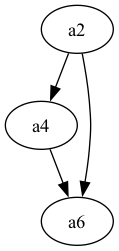
\includegraphics[width=.2\linewidth]{Imagens/safe_div_graph.png}
  \caption{Grafo de fluxo de controle}
  \label{fig:sub1}
\end{subfigure}%
\begin{subfigure}{.5\textwidth}
  \centering
  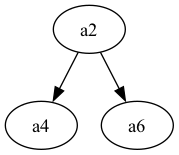
\includegraphics[width=.4\linewidth]{Imagens/safe_div_dominance.png}
  \caption{Árvore de dominância}
  \label{fig:sub2}
\end{subfigure}
\caption{CFG e Árvore de Dominância do Código de Divisão Segura}
\label{fig:graph-vs-dom-safe-div}
\small{Fonte: O autor}
\end{figure}

\begin{figure}[H]
\centering
\lstset{xleftmargin=.25\textwidth}
\begin{lstlisting}[language=haskell,style=nasm]
import Data.Bits

safe_div a0 a1 =
  let
    a2 () =
      let
        a3 = if a1 == 0 then 1 else 0
        a4 () =
          let
            a5 = a0 `div` a1
          in a6 a5
        a6 a7 =
          let
          in a7 
      in if a3 /= 0
        then a6 (-1)
        else a4 ()
  in a2 ()
\end{lstlisting}
\caption{Tradução Resultante do Exemplo de Divisão Segura}
\label{fig:safe-div-saida}
\small{Fonte: O autor, resultado dado pelo tradutor implementado}
\end{figure}

A Figura \ref{fig:safe-div-saida} contém o resultado da saída do tradutor implementado. Esse resultado é código Haskell e pode ser carregado no GHC e executado. Nota-se que na tradução as funções são equivalentes aos blocos da forma SSA: \verb|a2|, \verb|a4|, \verb|a6|. Com as funções \verb|a4| e \verb|a6| aninhadas a função \verb|a2|, visto que o bloco de \emph{label} \verb|2| domina imediatamente os outros blocos. Nota-se também que a função \verb|a6| tem um argumento, que corresponde a instrução \verb|phi| atribuída a \verb|%7|. Nas suas chamadas de cauda, \verb|a2| chama condicionalmente \verb|a6| com valor $-1$, e \verb|a4| usa como argumento a variável \verb|a5|.

\subsection{Algoritmo de Euclides}

Sendo $u$ e $v$ inteiros não nulos, o Maior Divisor Comum (GCD, do inglês \emph{Greatest Common Divisor}) é o maior inteiro que divide $u$ e $v$ sem deixar resto \cite{knuth2014art}. No Livro 7 de "Elementos" \ de Euclides, um algoritmo para calcular o GCD é descrito, que veio a ser conhecido como Algoritmo de Euclides. A Figura \ref{fig:euclides-cpp} apresenta uma implementação recursiva desse algoritmo na linguagem C, e esse código foi utilizado para gerar o exemplo de entrada em LLVM-IR da Figura \ref{fig:euclides-llvm}.

Este exemplo contém quatro blocos básicos: o bloco \verb|2| somente leva a execução ao bloco \verb|3|, no bloco \verb|3| há duas instruções \verb|phi| a comparação e um \emph{branch} que usa o valor da comparação, o bloco \verb|7| calcula o resto (\verb|srem|) e volta para o bloco \verb|3|, e por fim o bloco \verb|9| que somente faz o retorno do resultado armazenado na variável \verb|%4|. Neste exemplo há um um \emph{loop} entre os blocos \verb|a3| e \verb|a7|, que fica evidenciado no CFG na Figura \ref{fig:graph-vs-dom-gcd}, e que fica também explícito após a tradução nas chamadas de cauda das funções.

\begin{figure}[H]
    \centering
    \begin{subfigure}[b]{\textwidth}
        \centering
        \lstset{xleftmargin=.22\textwidth}
        \begin{lstlisting}[language=c,style=nasm]
int euclides_gcd(int a, int b) {
    if (b == 0) return a;
    else return euclides_gcd(b, a % b);
}
        \end{lstlisting}
        \caption{Algoritmo de Euclides em C}
        \label{fig:euclides-cpp}
    \end{subfigure}

    \vspace{1em} % Adds vertical space between the images

    \begin{subfigure}[b]{\textwidth}
        \begin{center}
        \lstset{xleftmargin=.20\textwidth}
        \begin{lstlisting}[language=llvm,style=nasm]
define i32 @euclides_gcd(i32 %0, i32 %1) {
2:
  br label %3

3:
  %4 = phi i32 [ %0, %2 ], [ %5, %7 ]
  %5 = phi i32 [ %1, %2 ], [ %8, %7 ]
  %6 = icmp eq i32 %5, 0
  br i1 %6, label %9, label %7

7:
  %8 = srem i32 %4, %5
  br label %3

9:
  ret i32 %4
}
        \end{lstlisting}
        \caption{Algoritmo de Euclides em LLVM-IR}
        \label{fig:euclides-llvm}
        \end{center}
    \end{subfigure}

    \vspace{.5em} % Adds vertical space between the images
    
    \caption{Algoritmo de Euclides em LLVM-IR}
    \label{fig:euclides-entrada}
    \small{Fonte: O autor, gerado usando \emph{clang} e editado}
\end{figure}

Segue do exemplo do Algoritmo de Euclides a tradução apresentada na Figura \ref{fig:euclides-saida}, com as quatro funções que correspondem aos quatro blocos da forma SSA. Destaca-se que a função \verb|a9| apenas retorna o valor recebido como argumento, assim como na forma SSA. As instruções \verb|phi| do bloco \verb|3| são traduzidos para os dois parâmetros da função \verb|a3|, e o valor que essa variável assume é definido dependendo de qual função está fazendo a chamada.

\begin{figure}[H]
\centering
\begin{subfigure}{.5\textwidth}
  \centering
  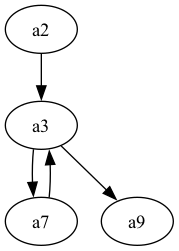
\includegraphics[width=.4\linewidth]{Imagens/gcd_graph.png}
  \caption{Grafo de fluxo de controle}
  \label{fig:sub1}
\end{subfigure}%
\begin{subfigure}{.5\textwidth}
  \centering
  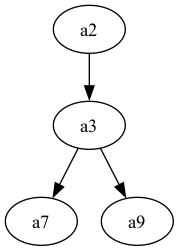
\includegraphics[width=.4\linewidth]{Imagens/gcd_dominance.png}
  \caption{Árvore de dominância}
  \label{fig:sub2}
\end{subfigure}
\caption{CFG e Árvore de Dominância do Código do Algoritmo de Euclides}
\label{fig:graph-vs-dom-gcd}
\small{Fonte: O autor}
\end{figure}

\begin{figure}[H]
\centering
\lstset{xleftmargin=.23\textwidth}
\begin{lstlisting}[language=haskell,style=nasm]
import Data.Bits

euclides_gcd a0 a1 =
  let
    a2 () =
      let
        a3 a4 a5 =
          let
            a6 = if a5 == 0 then 1 else 0
            a7 () =
              let
                a8 = a4 `mod` a5
              in a3 a5 a8
            a9 () =
              let
              in a4 
          in if a6 /= 0
            then a9 ()
            else a7 ()
      in a3 a0 a1
  in a2 ()
\end{lstlisting}
\caption{Tradução Resultante para o Exemplo do Algoritmo de Euclides}
\label{fig:euclides-saida}
\small{Fonte: O autor, resultado dado pelo tradutor implementado}
\end{figure}

\subsection{Teste de Primalidade}

Para obter um exemplo maior, foi utilizado um algoritmo \emph{naïve} de checagem de primalidade. O código da Figura \ref{fig:primo-c} recebe um inteiro \verb|num|, e se \verb|num <= 1| retorna \verb|0|, se não, faz um laço com \verb|i|, de dois até raiz quadrada de \verb|num| com passo um. E dentro da execução do laço, se \verb|num| é divisível por \verb|i| então \verb|num| não é primo. Se o laço de repetição termina sem retornar, então \verb|num| é primo.

\begin{figure}[h]
    \centering
    \begin{subfigure}[b]{\textwidth}
        \centering
        \lstset{xleftmargin=.2\textwidth}
        \begin{lstlisting}[language=c,style=nasm]
int is_prime(int num) {
    if (num <= 1) return 0;
    for (int i = 2; i * i <= num; i++) {
        if (num % i == 0) return 0;
    }
    return 1;
}
        \end{lstlisting}
        \caption{Teste de Primalidade \emph{Naïve} em C}
        \label{fig:primo-c}
    \end{subfigure}

    \vspace{1em} % Adds vertical space between the images

    \begin{subfigure}[b]{\textwidth}
        \begin{center}
        \lstset{xleftmargin=.21\textwidth}
        \begin{lstlisting}[language=llvm,style=nasm]
define i32 @is_prime(i32 %0) {
1:
  %2 = icmp slt i32 %0, 2
  br i1 %2, label %19, label %3

3:
  %4 = icmp slt i32 %0, 4
  %5 = and i32 %0, 1
  %6 = icmp eq i32 %5, 0
  %7 = or i1 %4, %6
  br i1 %7, label %16, label %8

8:
  %9 = phi i32 [ %10, %13 ], [ 2, %3 ]
  %10 = add nuw nsw i32 %9, 1
  %11 = mul nsw i32 %10, %10
  %12 = icmp sgt i32 %11, %0
  br i1 %12, label %16, label %13

13:
  %14 = srem i32 %0, %10
  %15 = icmp eq i32 %14, 0
  br i1 %15, label %16, label %8

16:
  %17 = phi i1 [ %4, %3 ], [ %12, %8 ], [ %12, %13 ]
  %18 = zext i1 %17 to i32
  br label %19

19:
  %20 = phi i32 [ 0, %1 ], [ %18, %16 ]
  ret i32 %20
}
        \end{lstlisting}
        \caption{Teste de Primalidade \emph{Naïve} em LLVM-IR}
        \end{center}
    \end{subfigure}

    \vspace{.5em} % Adds vertical space between the images
    
    \caption{Exemplo de Teste de Primalidade}
    \label{fig:primo-entrada}
    \small{Fonte: O autor, gerado usando \emph{clang} e editado}
\end{figure}

O código em LLVM-IR gerado a partir desse exemplo contém seis blocos, três dos quais \verb|8|, \verb|16| e \verb|19| tem instruções \verb|phi|. Observa-se que a instrução \verb|phi| atribuída a variável \verb|17| contém três argumentos, que acontece pelo fato de o fluxo chegar ao bloco \verb|16| a partir de outros três blocos e que o valor de \verb|17| é determinado pelo bloco que levou a execução até o \verb|16|. Nota-se na Figura \ref{fig:graph-vs-dom-prime} que esse exemplo contém um grafo de fluxo de controle mais notável, em que a árvore de dominância desempenha um papel importante ao apontar os escopos das variáveis e das funções após para a tradução.

Segue da aplicação da tradução nesse exemplo o resultado visto na Figura \ref{fig:primo-saida}. Código que contém seis funções, e pode-se perceber que as funções \verb|a8|, \verb|a16| e \verb|a19| têm suas instruções \verb|phi| traduzidas para seus argumentos. Pontua-se também que a variável \verb|%17|, que na forma SSA é atribuída à instrução \verb|phi| com três argumentos, e no código traduzido há três chamadas para a função \verb|a16|. Além disso, neste exemplo são usados operadores bit a bit, o "ou" \ (.|.) e o "e" \ (.\&.), que são definidos na biblioteca \verb|Data.Bits|.

Para comentar mais como a árvore de dominância é utilizada para definir o escopo das funções, pela Figura \ref{fig:graph-vs-dom-prime}, observa-se que o bloco \verb|a8| domina imediatamente somente o bloco \verb|a13|. Fazendo com que a função traduzida \verb|a13| exista somente dentro do escopo da função \verb|a8|.

\begin{figure}[h]
\centering
\lstset{xleftmargin=.16\textwidth}
\begin{lstlisting}[language=haskell,style=nasm]
import Data.Bits

is_prime a0 =
  let
    a1 () =
      let
        a2 = if a0 < 2 then 1 else 0
        a3 () =
          let
            a4 = if a0 < 4 then 1 else 0
            a5 = a0 .&. 1
            a6 = if a5 == 0 then 1 else 0
            a7 = a4 .|. a6
            a8 a9 =
              let
                a10 = a9 + 1
                a11 = a10 * a10
                a12 = if a11 > a0 then 1 else 0
                a13 () =
                  let
                    a14 = a0 `mod` a10
                    a15 = if a14 == 0 then 1 else 0
                  in if a15 /= 0
                    then a16 a12
                    else a8 a10
              in if a12 /= 0
                then a16 a12
                else a13 ()
            a16 a17 =
              let
                a18 = a17
              in a19 a18
          in if a7 /= 0
            then a16 a4
            else a8 2
        a19 a20 =
          let
          in a20 
      in if a2 /= 0
        then a19 0
        else a3 ()
  in a1 ()
\end{lstlisting}
\caption{Tradução Resultante do Exemplo de Teste de Primalidade}
\label{fig:primo-saida}
\small{Fonte: O autor}
\end{figure}

\begin{figure}[h]
\centering
\begin{subfigure}{.5\textwidth}
  \centering
  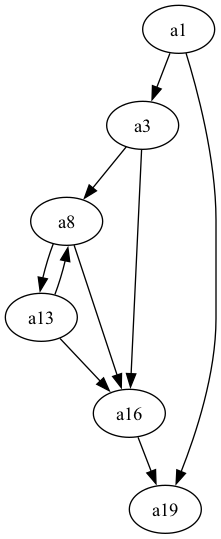
\includegraphics[width=.4\linewidth]{Imagens/prime_graph.png}
  \caption{Grafo de fluxo de controle}
\end{subfigure}%
\begin{subfigure}{.5\textwidth}
  \centering
  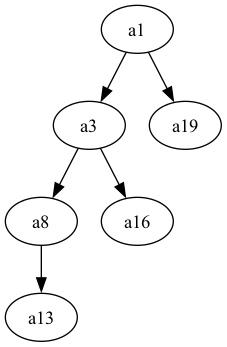
\includegraphics[width=.5\linewidth]{Imagens/prime_dominance.png}
  \caption{Árvore de dominância}
\end{subfigure}
\caption{CFG e Árvore de Dominância do Código de Teste de Primalidade}
\label{fig:graph-vs-dom-prime}
\small{Fonte: O autor}
\end{figure}

\section{Discussão}

Nessa seção será feita uma discussão sobre o que se mostrou possível traduzir através do método proposto. De início é possível comentar que a LLVM é um conjunto de ferramentas de tradução de código capaz de compilar projetos grandes com diversos arquivos, funções e bibliotecas. Porém nesse trabalho são traduzidas somente funções puras em um arquivo, permitindo também somente a chamada para outras funções puras. Além disso, como foi citado, a LLVM-IR conta com diversos tipos nativos e instrumentação robusta para definição de tipos compostos, enquanto que neste trabalho foram tratados somente de tipos inteiros simples.

Em termos: o método implementado nesse trabalho é capaz de traduzir funções puras que usam somente tipos inteiros simples de LLVM-IR para código Haskell em ANF. O fato de apenas funções puras serem traduzidas quer dizer que não foram tratados efeitos colaterais. Por exemplo: não são permitidas variáveis globais mutáveis, são compreendidos somente tipos inteiros simples (restringindo o uso de ponteiros de memória), não foi mapeada nenhuma chamada de sistema operacional, entre outras funcionalidades que fariam o uso de efeitos colaterais.

Desde a interpretação do código de entrada em LLVM-IR, por meio da definição da gramática livre de contexto, é garantida uma parte da pureza das funções. Isso se dá pois a gramática de entrada não permite variáveis globais, não mapeia operações que possam causar efeitos, e todas as instruções nativas da LLVM interpretadas são puras (sem mais efeitos além de receberem valores e retornarem um valor). Porém é importante pontuar que a imutabilidade das variáveis não é checada durante a tradução, mas para que o método possa traduzir corretamente, uma entrada válida em LLVM-IR é exigida.

Para estender a tradução e adicionar o tratamento de efeitos colaterais, pode ser estudado o uso da metalinguagem monádica apresentada por \citeonline{moggi1988computational}. Essa tese se fundamenta no fato de que, apesar de que \citeonline{sabry1992reasoning} estavam interessados em descobrir como aplicar otimizações tradicionais sem utilizar CPS quando introduziram o ANF, eles também demonstram que o cálculo obtido é equivalente ao cálculo-$\lambda$ computacional descrito por \citeonline{moggi1991notions}. Dada essa relação, e sabendo que, dessa forma, o cálculo usado pelo ANF é capaz de representar quaisquer efeitos computacionais, é possível estudar a definição de uma tradução sintática para a metalinguagem monádica de \citeonline{moggi1988computational}, o que permitiria a execução do código contendo efeitos colaterais dentro do GHC/Haskell.
